\documentclass[a4paper]{article}

\usepackage[francais]{babel}
\usepackage[utf8x]{inputenc}
\usepackage[T1]{fontenc}
%\usepackage{amsmath}
\usepackage{graphicx}
\usepackage[colorinlistoftodos]{todonotes}
\usepackage{comment}
\usepackage{float}
\usepackage[colorlinks=true,linkcolor=black,citecolor=black]{hyperref}
\usepackage{colortbl}

\frenchbsetup{StandardLists=true}

\title{\bsc{INSA} de Rennes \\ Département Informatique \\ \bigskip \hrule \bigskip ArchiPoilus \\ \bigskip Système d'annotation et de navigation dans des images d'archives \\ \bigskip Dossier de planification initiale \bigskip \hrule}
\author{Raphaël \bsc{Baron}, Pierre-Olivier \bsc{Bouteau}, Nicolas \bsc{Charpentier}, \\ Clément \bsc{Leboullenger}, Thomas \bsc{François}, Benoit \bsc{Travers}}

\begin{document}

\maketitle
\thispagestyle{empty}

\newpage
\tableofcontents
\thispagestyle{empty}

\newpage
\phantomsection
\addcontentsline{toc}{section}{Introduction}
\section*{Introduction}

	Les Archives départementales d'Ille-et-Vilaine sont en charge de la collecte, du classement, de la conservation et de la communication des archives qui constituent une grande partie du patrimoine historique écrit du département. 
\`A l'approche du centenaire de la Première Guerre Mondiale, les Archives, en collaboration avec l'\bsc{INSA} de Rennes, ont choisi de proposer aux étudiants en quatrième année du département informatique un sujet de mise en valeur des documents li\'es \`a la Grande Guerre.\\

	L'objectif du projet est de construire un outil d'annotations semi-auto\-matiques des documents liés au recrutement militaire concernant cette période. L'outil, dénommé ArchiPoilus, doit permettre à un utilisateur, visiteur des archives, d'associer lecture et annotation du document avec l'image numérisée qui lui correspond. En plus de naviguer et d'annoter les images, l'usager peut utiliser ces annotations pour rechercher des documents, par exemple trouver une personne grâce à son nom.\\
	
	Ce dossier de planification initiale présente notre projet dans les grandes lignes ainsi que la planifications des tâches à réaliser, tout en indiquant les dates consernant les livrables et les soutenances. Il contiendra notamment un premier diagramme de Gantt résumant graphiquement les intéractions et recouvrements temporels des tâches préalablement définies.\\
	
	Ce travail a fait l'objet d'échanges réguliers avec M. Jean-Yves Le Clerc, adjoint au directeur des Archives départementales d’Ille-et-Vilaine, afin de cibler au mieux les besoins auxquels devra répondre notre produit, et Mme. Karen Février, chef de projet chez ATOS, qui nous offre un suivi sur l'aspect gestion de projet ainsi que sur la rédaction des documents.

\newpage

\section{Présentation du projet : ArchiPoilus}

\subsection{Sujet}

	Dans le cadre des projets de 4\up{ème} année du département informatique, notre objectif est de développer une application permettant d’annoter des Registres Matricules Militaires (RMM) numérisés ainsi que leurs tables associées. Ces annotations doivent être à la fois simples et rapides à créer. Il sera important de pouvoir visualiser des images afin de pouvoir les annoter. De plus, l’application devra permettre à l’utilisateur de facilement rechercher des informations liées à ces annotations. Les principales fonctionnalités à développer seront la recherche de RMM, la visualisation d’images et l’annotation de ces images. Conformément au cahier des charges, notre application sera conçue pour fonctionner sur une table Microsoft PixelSense : nous utiliserons donc des émulateurs pour le développement du projet.\\
	
	Notre équipe est composée de 6 élèves ingénieurs de 4\up{ème} année du département informatique de l’INSA de Rennes : Raphaël \bsc{Baron}, Pierre-Olivier \bsc{Bouteau}, Nicolas \bsc{Charpentier}, Clément \bsc{Leboullenger}, Thomas \bsc{François} et Benoit \bsc{Travers}. Nous devons toutefois prendre en compte l’absence de Thomas et Benoit lors du second semestre pour cause de mobilité internationale; l’équipe sera donc réduite à quatre étudiants pour développer le projet pendant cette période.

\subsection{Mise en valeur des documents de guerre}

	L'application étant destinée à être utilisée dans le cadre du centenaire de la guerre 14-18, deux types de documents nous intéressent particulièrement : le registre matricule militaire et la table des registres matricules militaires. Ces documents ont été donnés aux archives par l'armée.

\subsubsection{Le registre matricule militaire}
	Le RMM (Registre Matricule Militaire), dont vous trouverez un exemple complet en annexe \ref{sec:annexe 1}, est un document qui récapitule la carrière d'un soldat. On peut notamment y trouver son état civil, c'est-à-dire son nom, son prénom, la date et le lieu de sa naissance et les noms de ses parents, ainsi que la description physique du soldat, le lieu de son engagement et ses différentes affectations. On y trouve aussi les campagnes auxquelles il a pris part, ainsi que ses éventuelles décorations et/ou condamnations.\\

	\`A la lumière du centenaire de la guerre 1914-1918, ces RMM prennent un intérêt particulier. En effet, ils permettent de déterminer quels soldats ont pris part à cette guerre, quelles batailles ils ont menées, et quel destin ils y ont trouvé. En bref, la valorisation du centenaire passe en grande partie par la mise en valeur de ces documents, qui seront mis en ligne par les archives d'Ille-et-Vilaine pour l'occasion.\\

	Le Registre Matricule Militaire est le document de base de notre projet. Afin de mieux le comprendre, celui-ci, étant divisé en plusieurs parties, est expliqué plus en détails dans notre rapport de pré-étude.\\

	Pour le RMM, il devra être possible, à travers l'application, de tout annoter, de n'importe quelle information présente dans le RMM jusqu'à l'annotation personnelle. 

\subsubsection{Les tables des registres matricules militaires}
	La table des RMM représente la liste de tous les registres présents dans un volume. Elle est triée par ordre alphabétique et permet donc de retrouver facilement un RMM, qui sont eux classés par numéros matricules croissants. Vous trouverez un exemple en annexe \ref{sec:annexe 2} où l'on peut trouver le matricule et donc le RMM de l'individu nommé Onen (annexe \ref{sec:annexe 1}).\\

	Ces tables nous seront utiles pour la rapidité de recherche de l'information. En effet, le numéro matricule est un moyen de recherche efficace puisqu'ils sont rangés, dans un volume, en ordre numérique. \\

	L'objectif de l'application sera donc d'offrir la possibilité de naviguer d'une table à un RMM directement en rendant donc la zone du numéro matricule "cliquable" tel un lien hypertexte.\\

\section{Spécifications fonctionnelles}

	L’application possédera cinq principales interfaces / écrans dont voici le schéma de navigation (figure \ref{fig:navigation}). On y retrouve une interface d'accueil permettant à l'utilisateur de s'authentifier, l'interface de recherche qui facilite la recherche de tables et de RMM, l'interface de gestion des documents, ainsi que deux interfaces de visualisation, une pour les tables et une autre pour les RMM.

\begin{figure}[H]
\centering
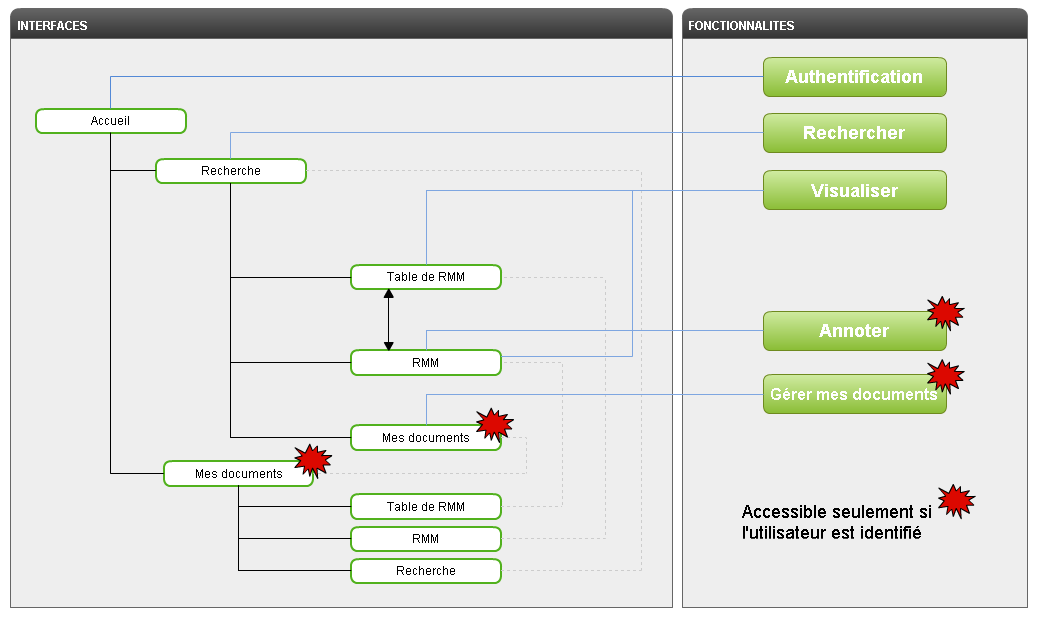
\includegraphics[width=\textwidth]{navigation.png}
\caption{Schéma de navigation de l'application}
\label{fig:navigation}
\end{figure}

	Lorsque l’utilisateur commencera à utiliser l’application, celui-ci se retrouvera sur un écran d’accueil qui lui proposera deux fonctionnalités : s'inscrire ou bien s’identifier. De plus, un écran de recherche devra être accessible à partir de n’importe quel autre écran permettant à l'utilisateur d'effectuer une recherche. La gestion des documents ne seront accessibles que si l’utilisateur est déjà identifié. Les écrans de visualisation de document pourront être accessibles à partir d’une recherche ou bien lorsque l’utilisateur souhaite consulter un de ses documents. Aussi, à partir d’une visualisation de table, il sera possible à l’utilisateur d’accéder à un ou plusieurs RMM.\\
	
	La phase de développement de cette application passe par le développement de 6 fonctionnalités : l'authentification d'un utilisateur, la recherche de document, la navigation entre différents documents, la visualisation de documents, l'annotation de documents et enfin la gestion des différents types d'utilisateurs. Pour plus d'information concernant le détails de ces spécifications, nous vous invitons à lire notre rapport de spécification fonctionnelle.\\
	
\section{Méthodologie}

	\subsection{Gestionnaire de version}

	Pour améliorer notre efficacité lors de rédaction de rapports, nous utilisons un gestionnaire de versions Git. Nous avons créé un dépôt sur GitHub qui est un service web d'hébergement et de gestion de développement de logiciels, utilisant Git. Celui-ci nous permet de travailler en même temps sur un même document. Le possible inconvénient d'utiliser ce genre de logiciel est de posséder une connexion internet permanente et de prévoir un temps de prise en main pour chacune des ressources. Mais l'avantage est un gain de temps non négligeable en matière de rassemblement de travaux et de mise en commun. De plus, lorsque nous passerons au codage de notre solution, cet outil sera alors quasiment indispensable.

	\subsection{Cycle en V}
	
	Pour mener à bien notre projet, nous avons choisi de suivre un cycle en V par rapport à une méthode agile pour plusieurs raisons.\\
	
	La méthode agile est adaptée aux projets de développement en informatique. Elle permet de mener un projet par incréments : elle consiste à mettre au point un produit rapidement puis de l'améliorer en prenant en compte les avis des différents clients/utilisateurs. Cependant, cette méthode nécessite de faire des nombreuses et courtes itérations et le temps qui nous est imparti pour réaliser le projet ne nous permet pas de faire plusieurs itérations. Or ce sont ces itérations successives qui font tout l'intérêt de la méthode.\\
	
	Les nombreux livrables ont des dates imposées et l'enchaînement des livrables correspond au développement d'un projet suivant un cycle en V. C'est pourquoi nous suivons cette méthode de planification. La figure suivante montre les différentes phases d'un cycle en V (figure 2).\\
	
\begin{figure}[H]
\centering
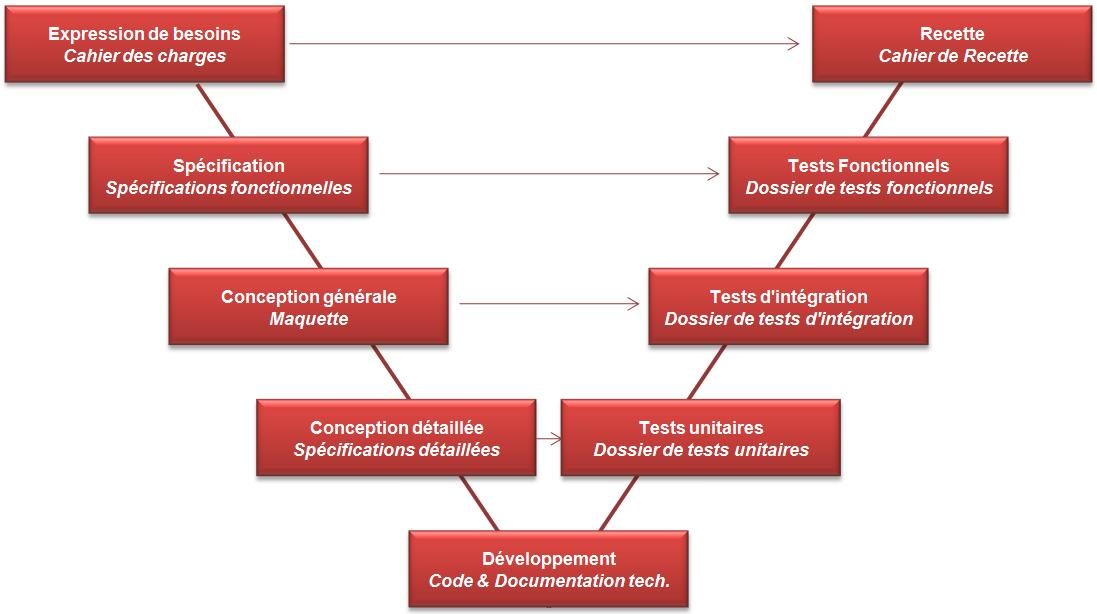
\includegraphics[width=\textwidth]{Cycle_en_V.jpg}
\caption{Cycle en V}
\label{fig:cycleenv}
\end{figure}
	
	Actuellement nous sommes entre la phase de spécification et de conception du système. L'expression des besoins à été réalisée lors des échanges avec les Archives départementales d’Ille-et-Vilaine.
	
\subsection{Chronologie}

	La prochaine phase du projet est la conception logicielle. Sachant qu'il va être difficile de travailler pendant les congés de Noël et que des partiels nous occuperons début Janvier, nous avons prévu de commencer la prochaine phase du projet le 20 Janvier. La chronologie suivante (figure 3) montre les phases du projet (conception logicielle - prise en main - développement - livraison) avec les dates des différents livrables et soutenances associés. La phase de développement comprend le codage de chaque spécification fonctionnelle (la case "SF -" n'est pas complète et correspond à "SF - Administration"). En fin de projet, une longue période est réservée pour la rédaction de rapport et la préparation de soutenance. En effet, des partiels en mai ne nous permettent pas de consacrer beaucoup de temps au projet, c'est pour cela que cette période est assez longue.
	
\begin{figure}[H]
\centering
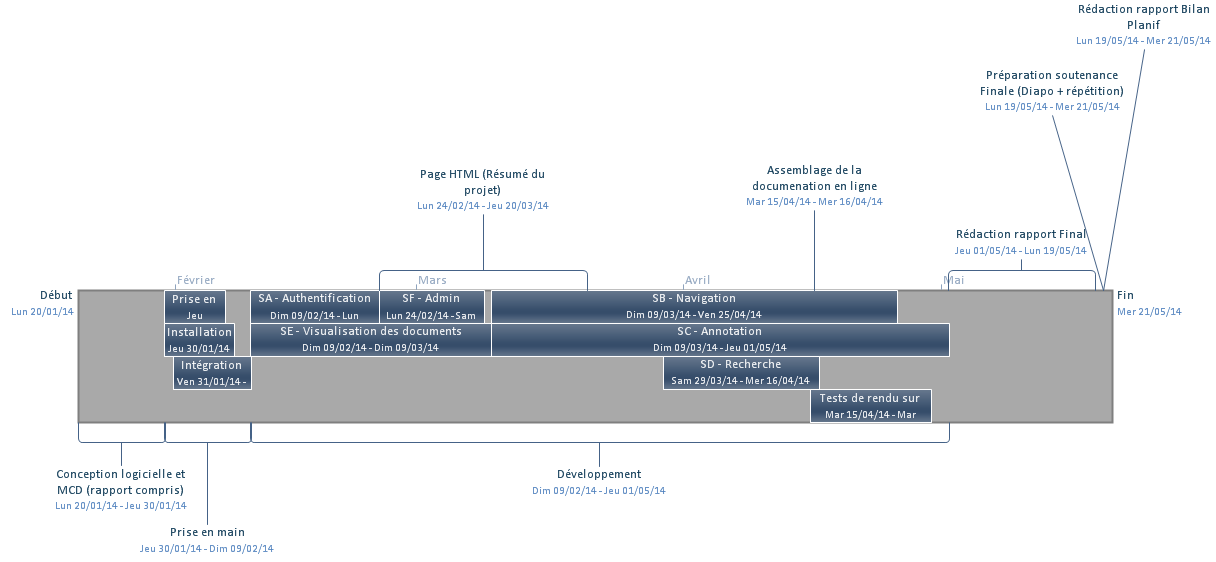
\includegraphics[width=\textwidth]{chronologie.png}
\caption{Chronologie du projet}
\label{fig:chronologie}
\end{figure}

	Dates des livrables :

\begin{itemize}
\item Rapport de conception logicielle : 13 Février
\item Page HTML (résumé du projet) : 3 Avril
\item Documentation en ligne du logiciel : 28 Mai
\item Rapport Final, Annexes et Rapport de bilan de planification : 21 Mai
\end{itemize}

	Date de la soutenance finale de projet : 27-28 Mai\\

\subsection{Diagramme de Gantt}

	Le diagramme de Gantt suivant (figure 4) montre en détail la planification des tâches restantes pour le projet.

\begin{figure}[H]
\centering
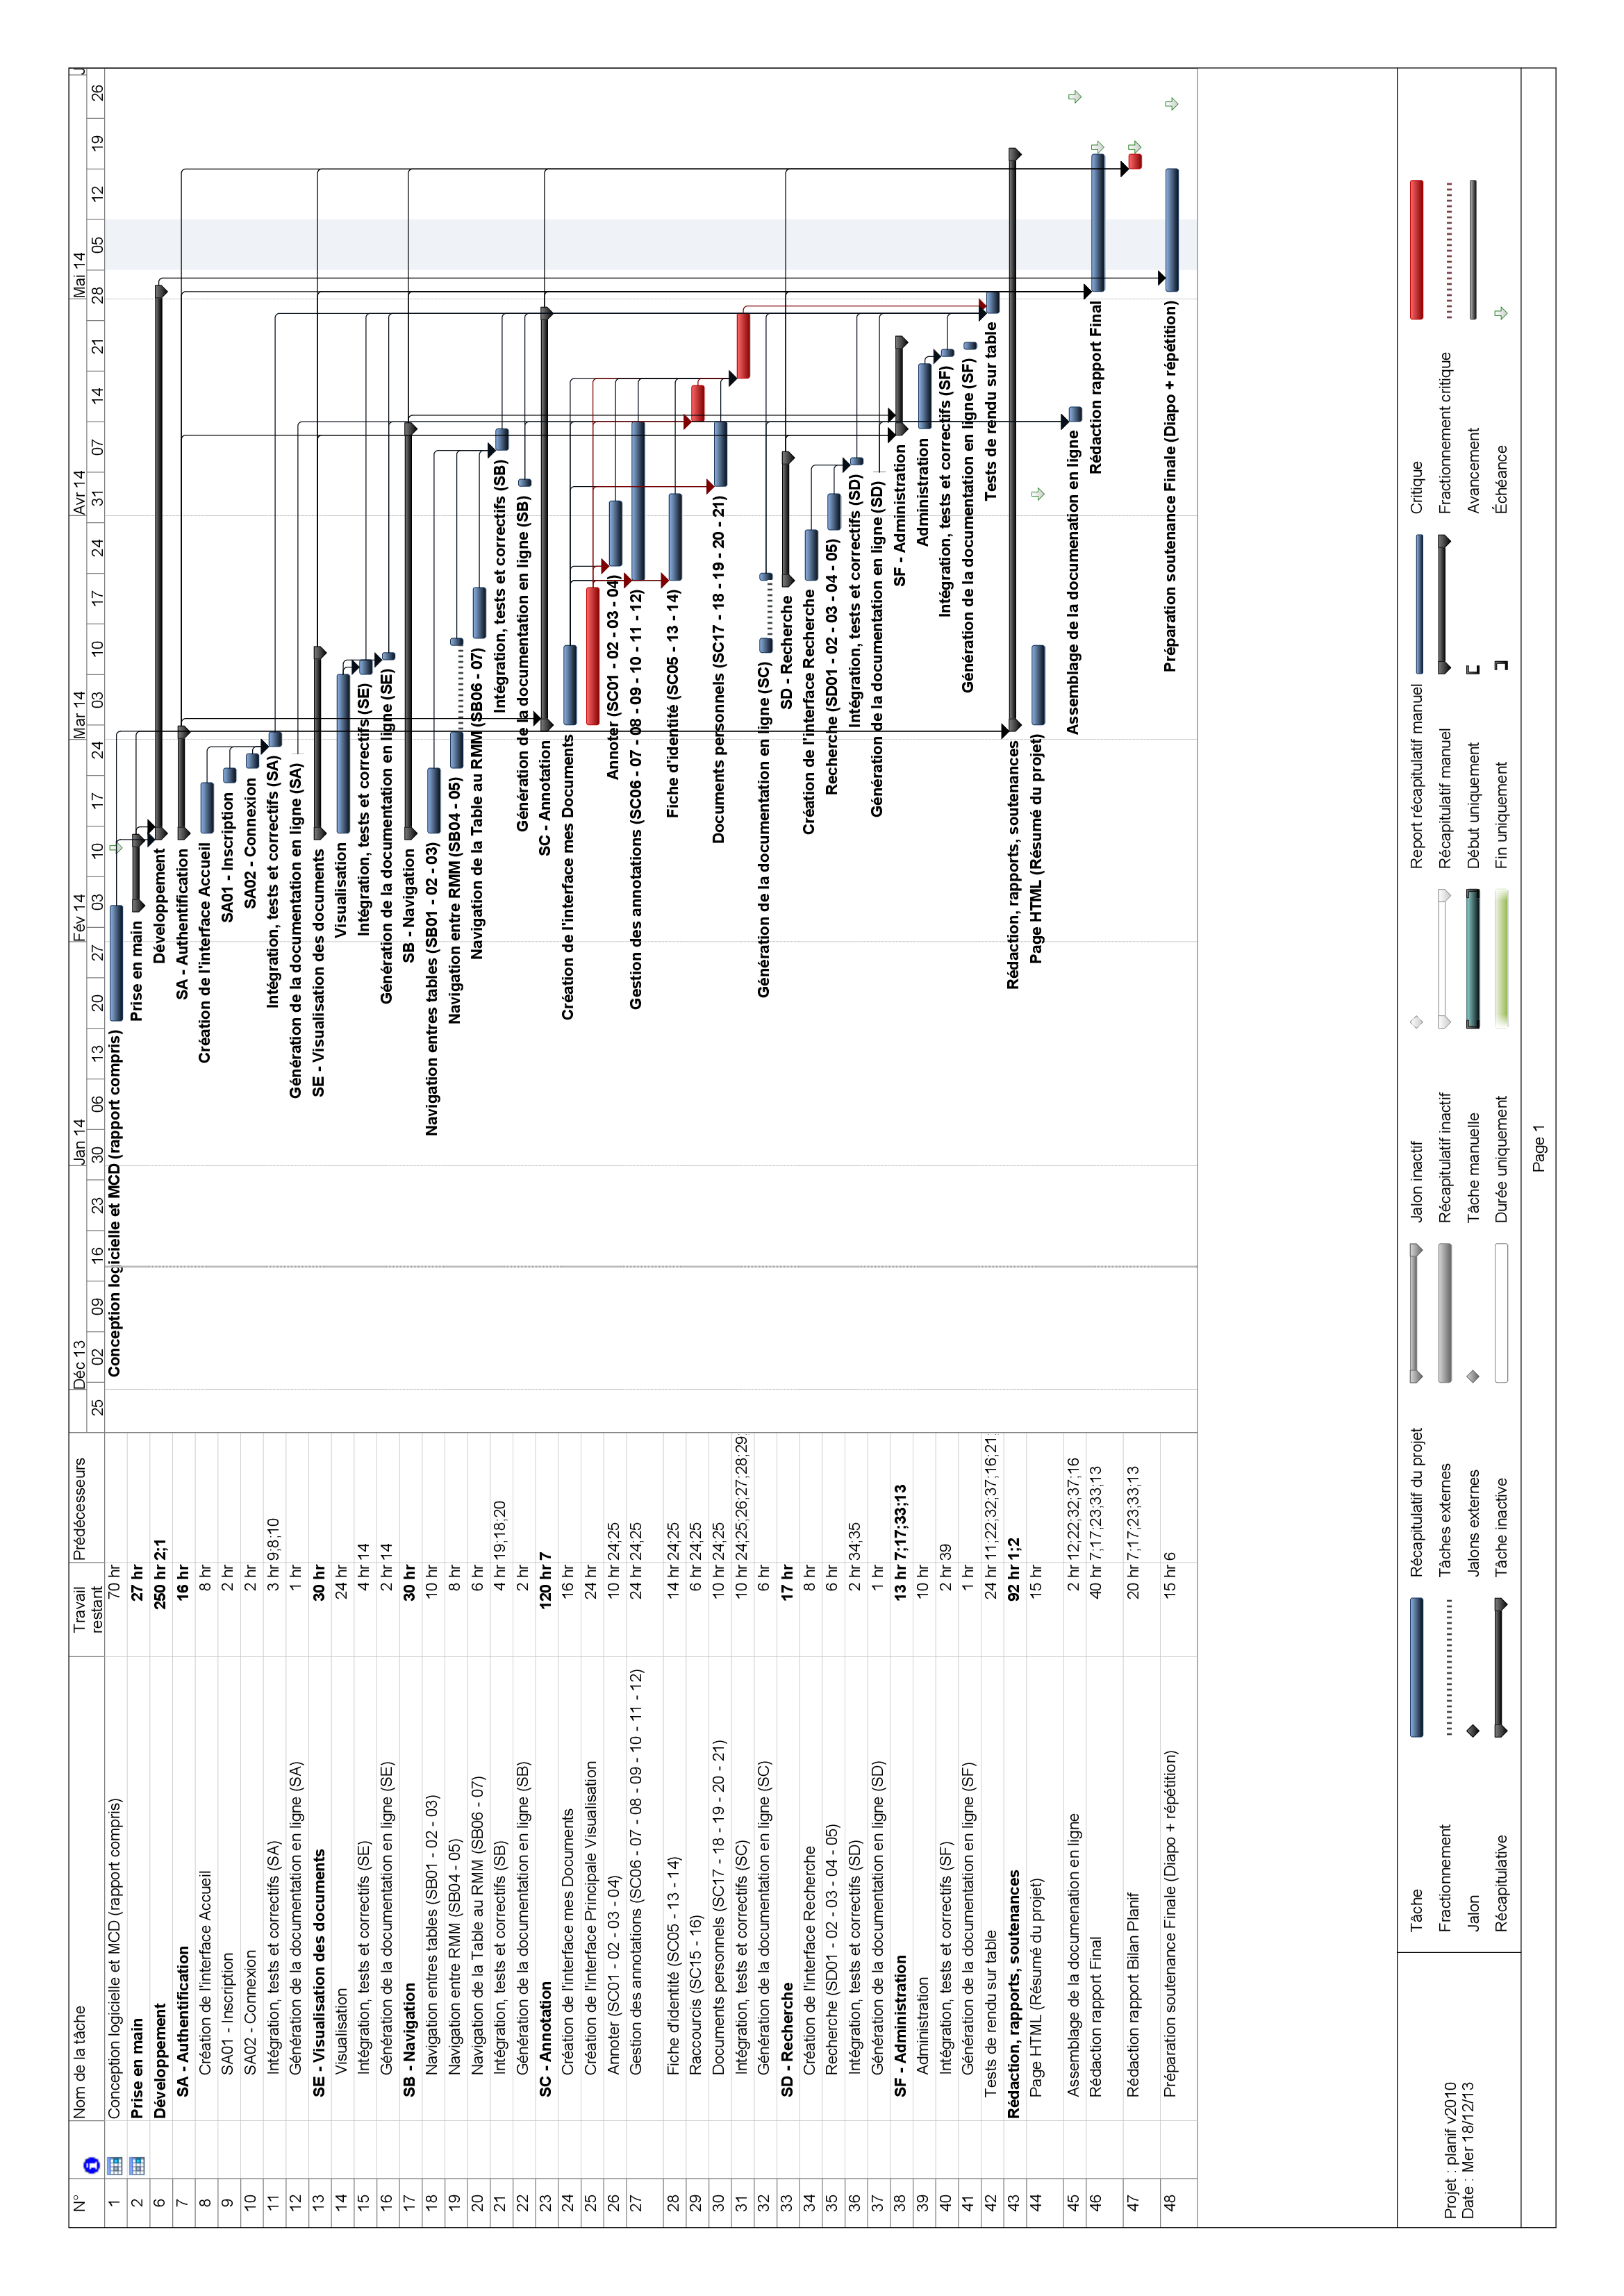
\includegraphics[width=\textwidth]{gantt.png}
\caption{Diagramme de Gantt}
\label{fig:gantt}
\end{figure}

\newpage

	Pour chaque tâche, nous avons affecté une ressource unique, c'est-à-dire qu'une tâche va être effectuée par une seule personne. Ceci explique le fait que certaines tâches soient effectuées en parallèle. De plus, nous avons estimé le nombre d'heures de travail hebdomadaire, à savoir : 
	
\begin{itemize}
\item 5 heures de travail par personne par semaine pour les semaines classiques
\item 10 heures de travail par personne par semaine lors des congés (congés de Mars et d'Avril)
\item 15 heures de travail par personne par semaine lors de la semaine réservé au projet en Mai
\item Pas de travail sur le projet du lundi 5 Mai au vendredi 16 Mai (partiels)
\end{itemize}

	Nous avons au total environ 420 heures disponibles pour travailler le projet, qui sont en adéquation avec les 414 heures de prévues par la planification.\\

	On peut remarquer que la phase de développement se termine au début du mois de Mai, et nous allons proposer aux Archives départementales d’Ille-et-Vilaine de tester notre produit au début du mois de Mai. Cela nous permettra d'avoir des avis sur notre application afin de pouvoir faire des améliorations.\\

	Afin de réaliser une première version à la fois fonctionnelle et à valeur ajoutée par rapport aux produits existants, nous avons priorisé les tâches. Sachant que le système ne nécessite pas la gestion des différents utilisateurs pour fonctionner, cette tâche est définie comme moins prioritaire et est donc placée en dernière. Selon notre estimation des charges et notre estimation du temps disponible, nous devrions pouvoir réaliser toutes les fonctionnalités dans le temps imparti. Mais nous ne sommes pas à l'abri d'un problème technique, humain ou même d'une mauvaise estimation du temps de réalisation. C'est pourquoi la gestion des différents utilisateurs peut être omise par manque de temps.\\
	
	Pour le déroulement du projet, il conviendra de mettre à jour ce diagramme de Gantt et de vérifier régulièrement si les délais sont respectés.

\newpage
\phantomsection
\addcontentsline{toc}{section}{Conclusion}
\section*{Conclusion}

	Dans la perspective du centenaire de la guerre 14-18, ce projet a pour objectif de concevoir un outil en ligne multi-utilisateurs de navigation et d’annotation des RMM sur un support tactile.\\
	
	Le développement de notre application, ArchiPoilus, suit un Cycle en V. En effet, c'est pour nous la méthode de planification la plus adpatée à ce projet puisque ses différentes phases correspondent exactement avec les dates des livrables à fournir. Le diagramme de Gantt montre la répartition des tâches pour la suite du projet. Il faudra régulièrement vérifier si l'estimation du temps à consacrer à chaque tâche est exacte, si on prend du retard par rapport au planning et tenir le cas échéant le diagramme de Gantt à jour.\\
	
	Depuis le commencement du projet, nous travaillons en collaboration avec M. Jean-Yves Le Clerc, adjoint au directeur des Archives départementales d’Ille-et-Vilaine, afin de cibler au mieux les besoins auxquels devra répondre notre produit. Nous allons proposer aux Archives départementales d’Ille-et-Vilaine de tester notre application afin d'intégrer des améliorations en fin de projet. Nous souhaitons garder cette "relation client"  pour la suite du projet, qui nous offre l’opportunité de travailler avec des professionnels.\\
	
	Aussi, nous bénéficions du suivi de Mme Karen Février, chef de projet chez ATOS, sur l’aspect gestion de projet, que nous remercions pour ces nombreux retours depuis le début du projet, et en particulier sur la planification du projet.\\
	
	La prochaine phase de notre projet est la conception logicielle de notre application. Elle permettra de préparer au mieux la phase de développement.

\appendix

\section{Vue compl\`ete d'un RMM}
\label{sec:annexe 1}

\begin{figure}[H]
\centering
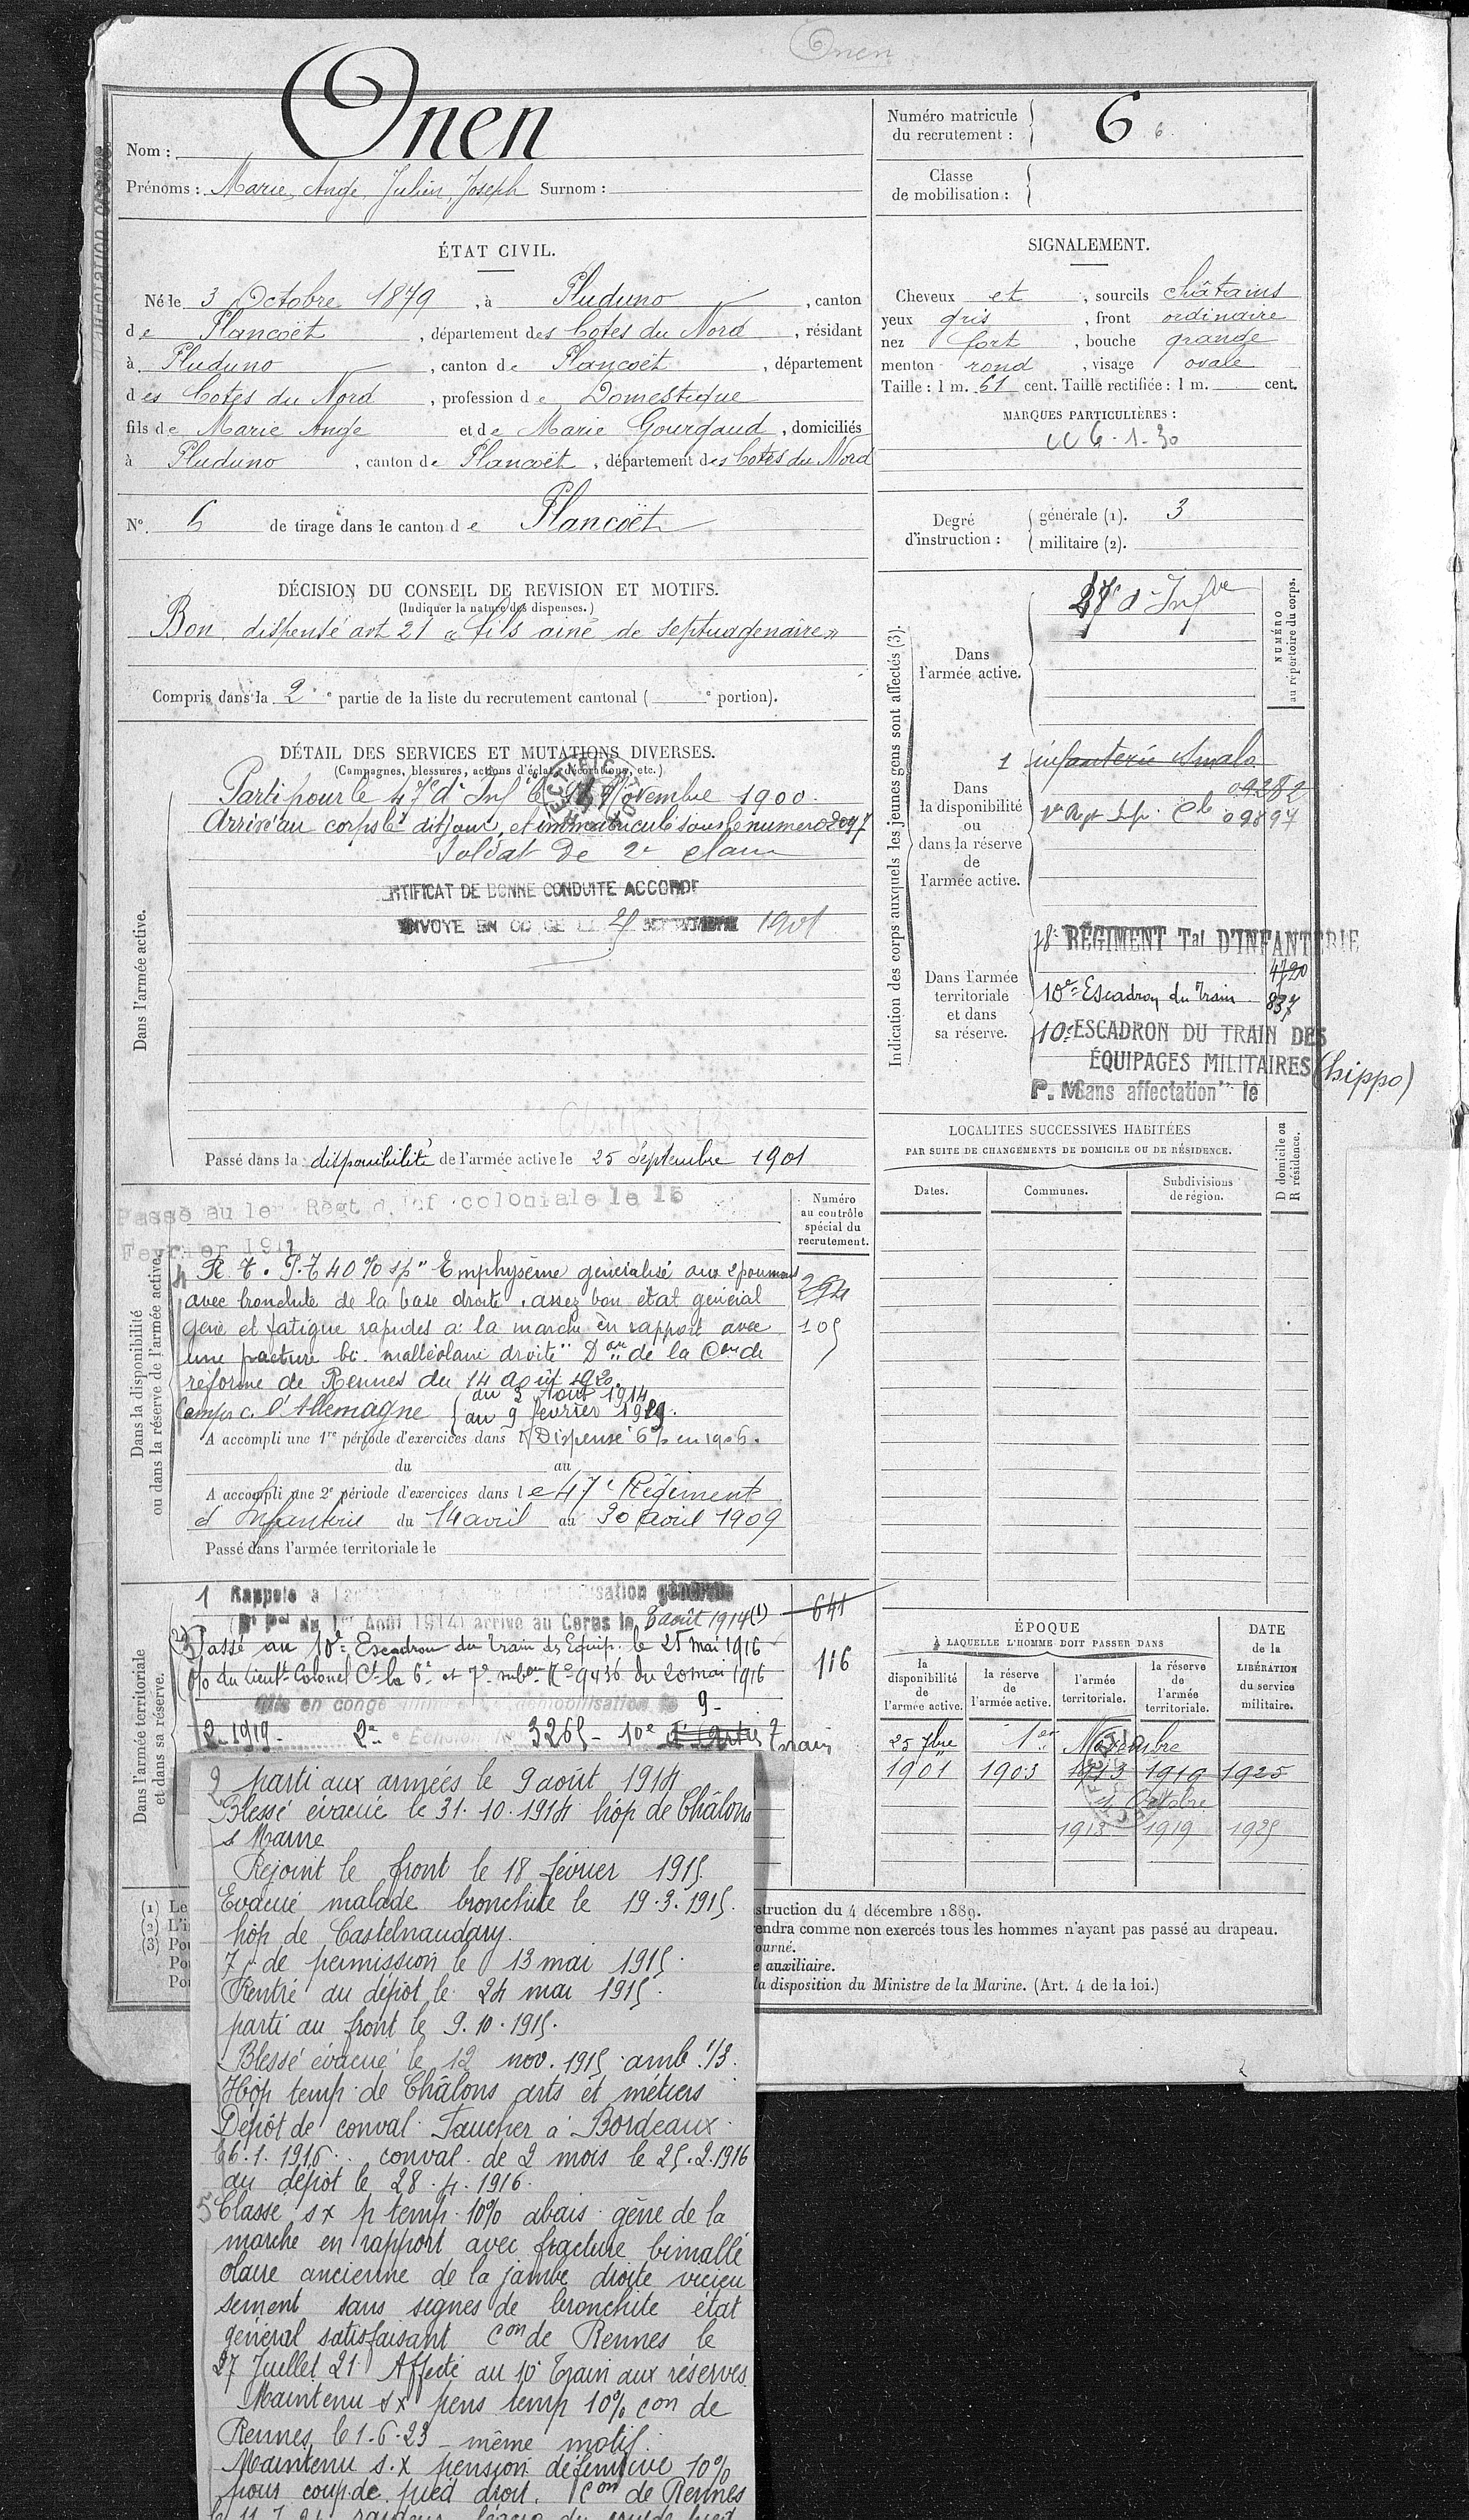
\includegraphics[width=0.95\textwidth]{RMM.JPG}
\end{figure}

\section{Table de RMM - Saint-Malo 1899}
\label{sec:annexe 2}

\begin{figure}[H]
\centering
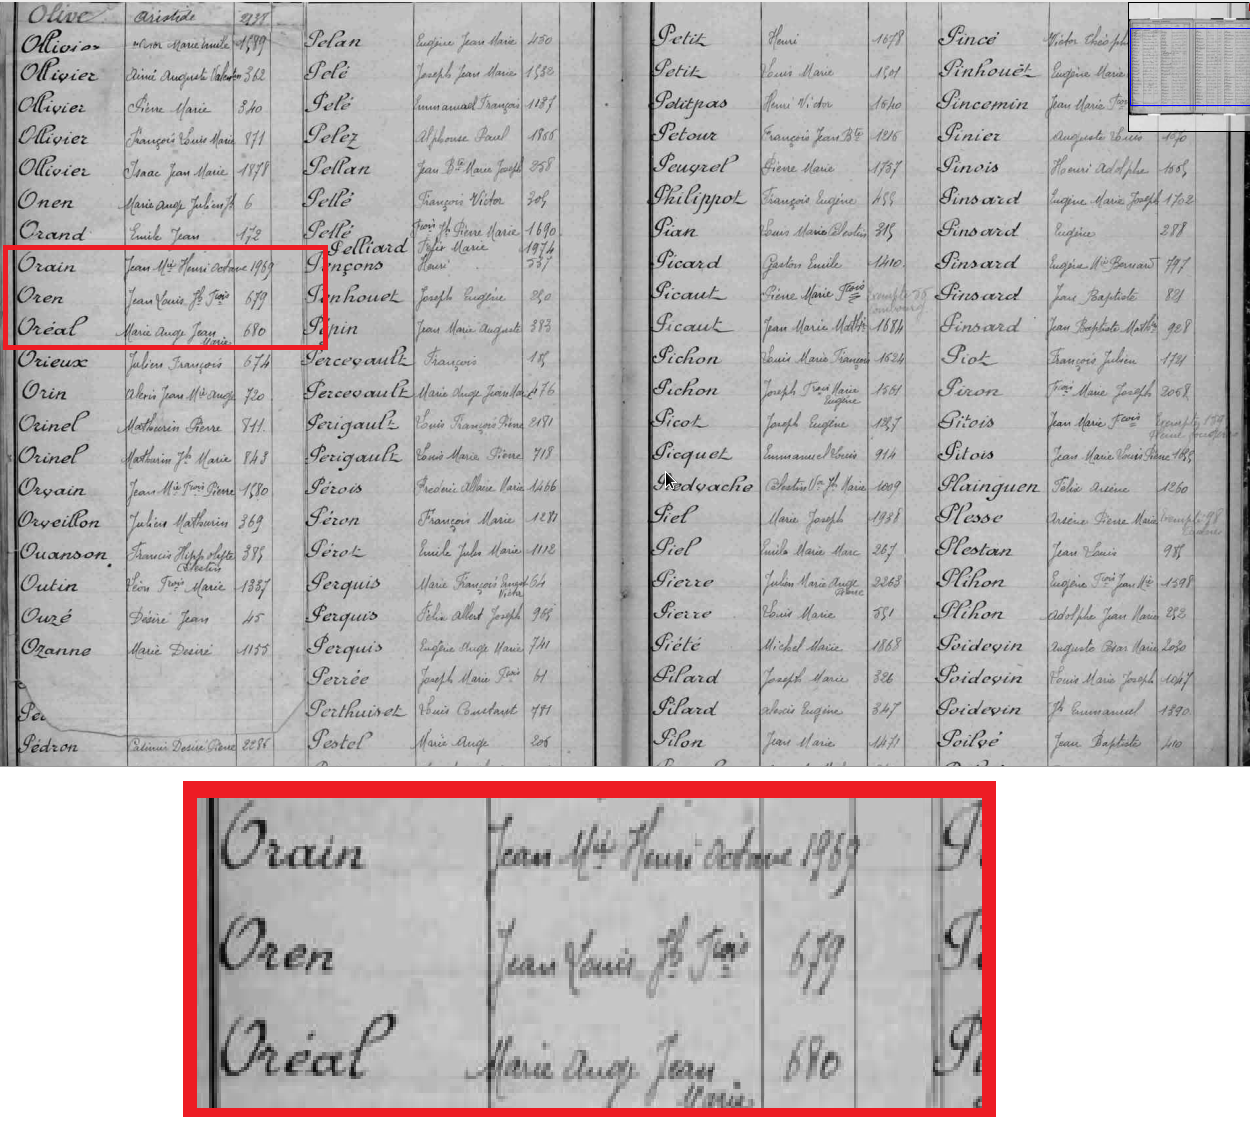
\includegraphics[width=\textwidth]{Table_Onen.png}
\end{figure}

\end{document}
